\documentclass[12pt,francais]{report}

\usepackage[UTF8]{inputenc}
\usepackage[pdftex]{graphicx}
\usepackage[french]{babel}
\usepackage{enumitem}
\usepackage{scrextend}
\usepackage{float} 

\begin{document}

\begin{center}

\includegraphics[scale=0.3]{./images/logo_universite_orleans.png}~\\[1.5cm]

\textsc{\large Master 1 - TER}\\[1cm]	

\rule{\linewidth}{0.5mm}\\[0.4cm]

{ \LARGE \bfseries GoodLua\\[0.4cm] }

\rule{\linewidth}{0.5mm}\\[2cm]
\end{center}


\begin{minipage}{0.4\textwidth}
      \begin{flushleft}
			\textsc{Bovie} Pierre-Edouard\\
			\textsc{Labourbe} Loïc\\
			\textsc{Maslowski} Antoine\\
			\textsc{Roche} Julie\\
			\end{flushleft}
    \end{minipage}\hfill
    \begin{minipage}{0.6\textwidth}
      \begin{flushright}
			Enseignants : \textsc{Couvreur} Jean-Michel\\
			\textsc{Dabrowski} Frederic\\

\end{flushright}
    \end{minipage}\\[1.5cm]
		
		\begin{center}
    {7 Février 2018 - 25 Mai 2018}
		\end{center}
		
\chapter*{Résumé du projet}

L’objet du projet est la conception d'un système pour la création et le lancement à distance de programme Lua s'exécutant sur un robot. Le système matériel est composé d'une tablette Androïd et '’un robot mobile à base pcDuino équipé de divers capteurs. Le logiciel de la tablette offrira la possibilité : 
\begin{itemize}
\item de concevoir des programmes
\item de charger à distance le programme sur le robot 
\item de télécommander le robot 
\end{itemize} 
Le système logiciel sur le robot permettra de recevoir et d'exécuter les programmes Lua transmis par la tablette.

\chapter*{Introduction au domaine}

\chapter*{Besoins fonctionnels}

\begin{itemize}[label=\textbullet]
	\item \textbf{exécuter du code}
	\begin{description}
		\item \textit{description :} exécuter du code eLua sur le PcDuino
		\item \textit{priorité :} très haute
		\item \textit{justification :} cette fonctionnalité est la principale. Nous devons être en mesure de faire fonctionner le robot grâce à du code eLua avant toute autre chose.
	\end{description}
	\item \textbf{connecter android au robot grâce au wifi}
	\begin{description}
		\item \textit{description :} utiliser la carte wifi du PcDuino pour la connecter à un appareil androïd.
		\item \textit{priorité :} haute
		\item \textit{justification :} le code crée via l'application androïd doit être transmis au robot pour être exécuté. Une solution filaire étant peu pratique, nous le connecterons via wifi.
	\end{description}
	\item \textbf{transformer blockly en eLua}
	\begin{description}
		\item \textit{description :} traduire les blocs de la librairie Blockly dans le langage Lua, plus spécifiquement en eLua.
		\item \textit{priorité :} moyenne
		\item \textit{justification :} le robot étant "guidé" par du code eLua, il est nécessaire de procéder à une traduction du programme visuel dans ce langage avant de l'envoyer au robot pour être exécuté.
	\end{description}
	\item \textbf{créer un programme}
	\begin{description}
		\item \textit{description :} la création d'un nouveau programme blockly via l'application androïd.
		\item \textit{priorité :} moyenne
		\item \textit{justification :} c'est la fonctionnalité de base de l'application, il faut pouvoir créer de nouveaux programmes en vue de les écrire et de les exécuter.
	\end{description}
	\item \textbf{sauvegarder / charger des programmes}
	\begin{description}
		\item \textit{description :} l'utilisateur pourra sauvegarder les programmes sur lesquels il travaille, et reprendre sa progression là où il était en chargeant un programme parmi ceux enregistrés.
		\item \textit{priorité :} basse
		\item \textit{justification :} cela permettra de travailler sur un programme en plusieurs fois sans risque de perdre son travail. Cette fonctionnalité était à la base en option, mais l'architecture de notre application nécessite de pouvoir l'utiliser.
	\end{description}
\end{itemize}

\bigskip
\textbf{Prototype - l'interface de l'application Androïd :}\\
En ouvrant l'application, l'utilisateur se verra proposer de créer un nouveau programme, il devra alors lui donner un nom, ou alors de charger un programme déjà existant, en choisissant dans une liste. Une fois le programme sélectionné ou créé, il aura le choix de le modifier ou de l'exécuter. [Figure 1]

Dans le cas du choix de modifier le code, on ouvrira l'éditeur visuel contenant Blockly avec l'ensemble des blocs disponibles dans une barre latérale gauche. Un menu permettra également de sauvegarder le programme en cours d'édition ou de l'effacer. [Figure 2]\\

\begin{figure}[!h]
\begin{addmargin}[-7em]{1em}
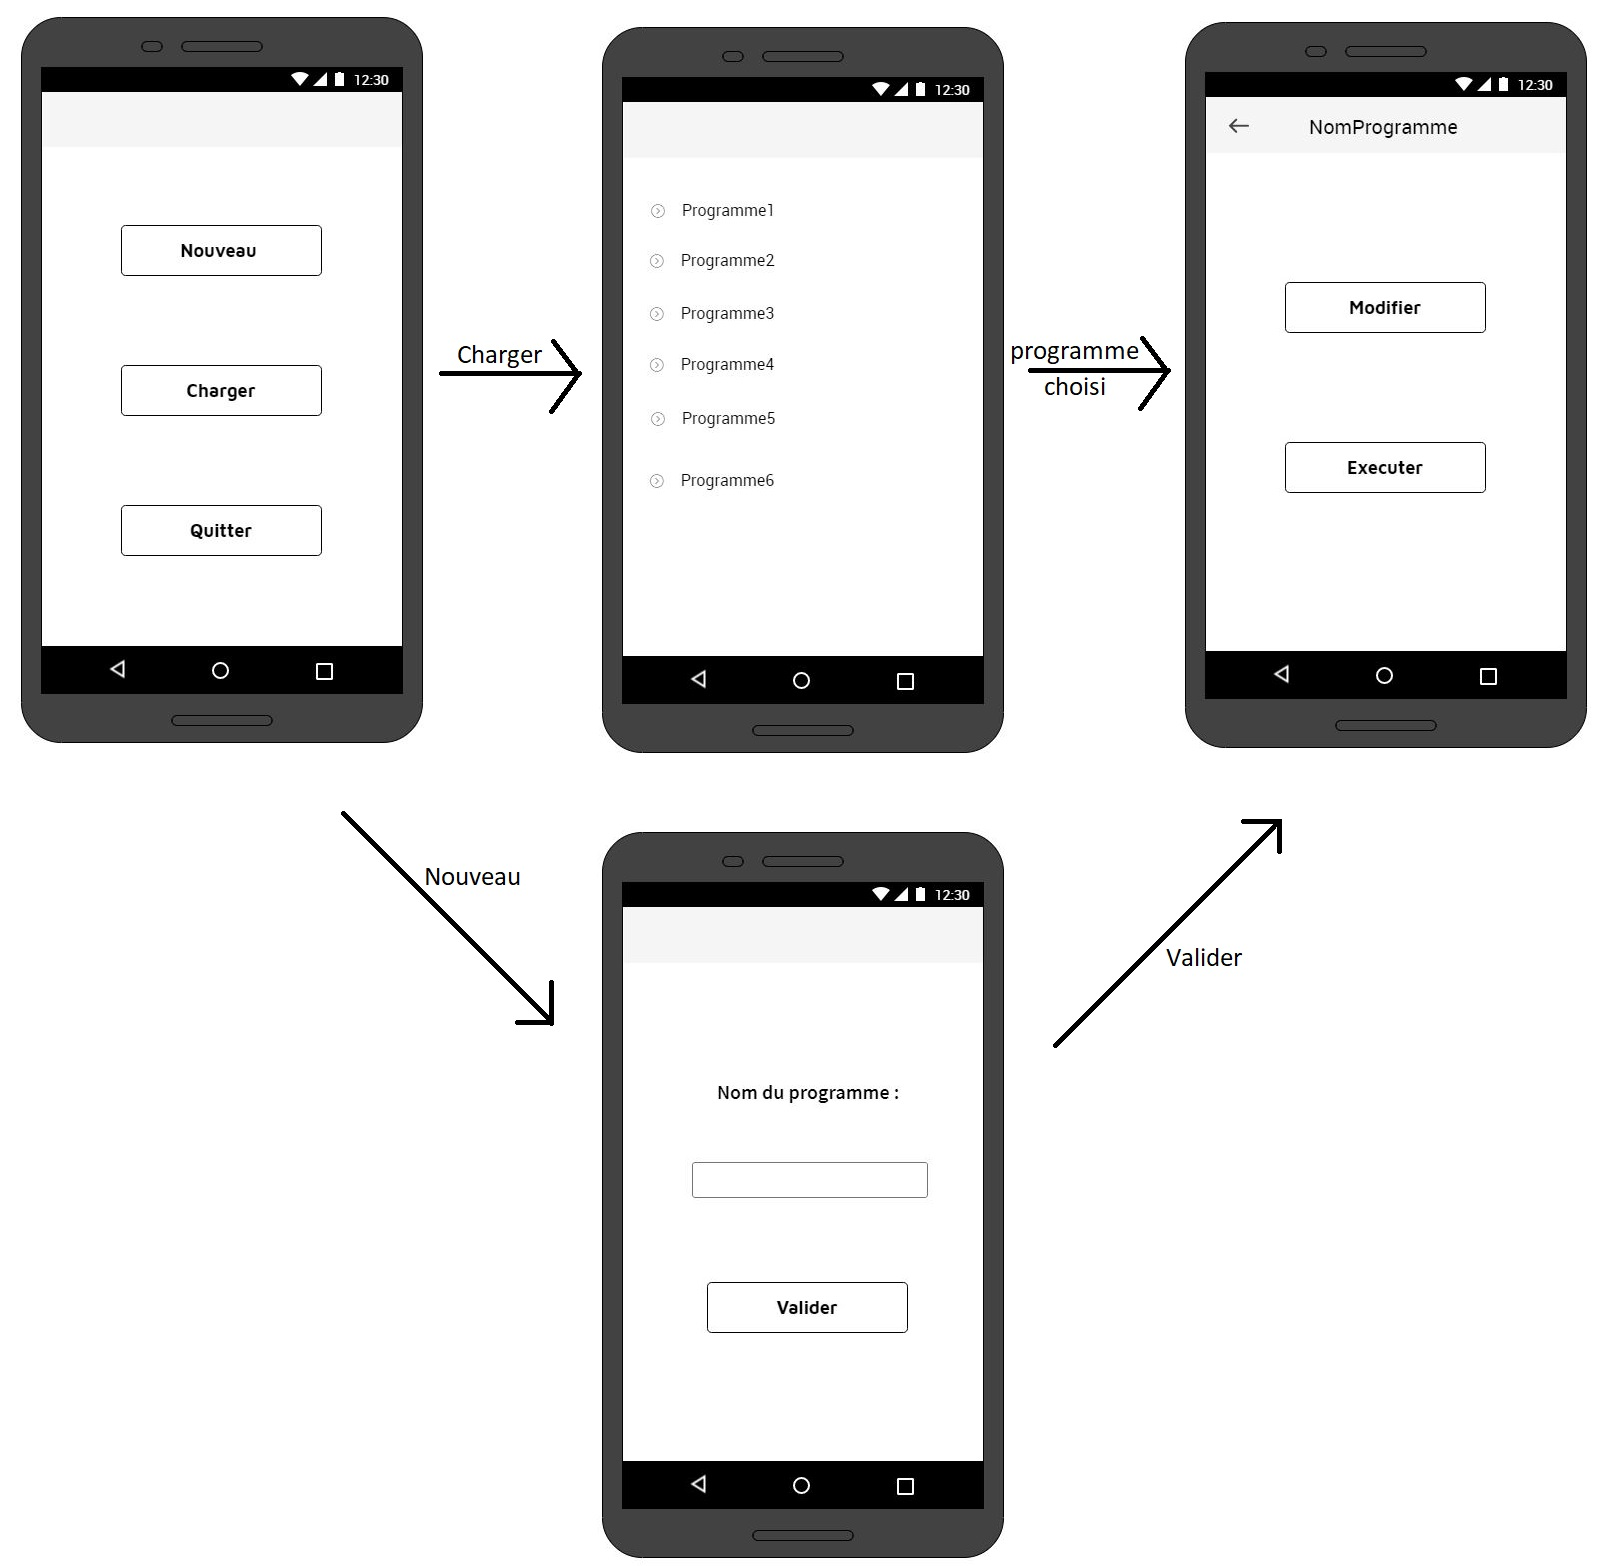
\includegraphics[scale=0.45]{./images/maquette1.jpg}~\\[1.5cm]
\caption{Maquette 1ère partie}
\end{addmargin}
\end{figure}

\begin{figure}[!h]
\begin{addmargin}[-5em]{1em}
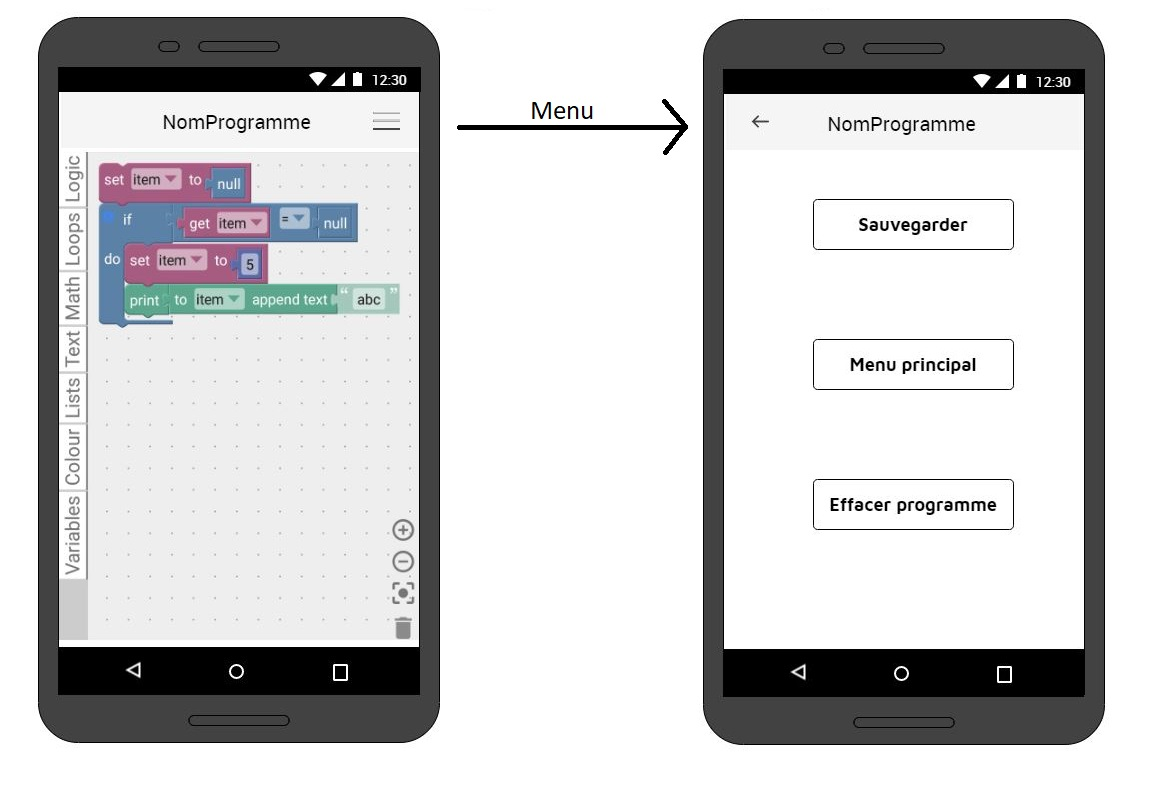
\includegraphics[scale=0.6]{./images/maquette2.jpg}~\\[1.5cm]
\caption{Maquette 2ème partie}
\end{addmargin}
\end{figure}




\chapter*{Besoins non fonctionnels}

\begin{description}
	\item [environnement de travail :]Nous travaillons sous une distribution Ubuntu. Pour la partie programmation en eLua, il est possible d'utiliser n'importe quel éditeur de texte, puis de compiler le fichier.
	\item [exécution en temps réel / rapidité :] Il serait préférable que l'exécution d'un programme se fasse de manière assez rapide, pour ne pas aller contre les attentes de l'utilisateur. Par exemple, si le programme utilise des capteurs, mais qu'une lenteur dans le programme fait qu'un obstacle n'est pas détecté à temps, cela nuira à l'expérience de l'utilisateur. De même, l'un des buts de l'application, est de pouvoir exécuter une séquence, ou de donner des ordres au robot en temps réel.
	\item [simplicité d'utilisation : ]L'application doit être utilisable par des utilisateurs sachant programmer, qui pourront créer un programme complexe à partir des blocs basiques, mais elle doit également être accessible à des utilisateurs débutants en programmation, qui pourront utiliser des blocs représentant des fonctions toutes faites concernant le robot (par exemple : allumer LED). Les blocs et l'interface devront donc être instinctifs et simples d'utilisation.
\end{description}


\chapter*{Analyse de l'existant}

Nous avons reçu pour ce projet, un kit matériel qui forme le robot.\\
Pour nous aider à découvrir son utilisation, nous avons étudié le projet d'algorithmique répartie des étudiants de la promotion 2015 des master 1 informatique \cite{ref1} dans lequel ils manipulent un robot semblable au notre, mais avec des des langages différent du notre (eLua) puisqu'ils l'ont contrôlé avec du python et du C++.

\begin{figure}[!h]
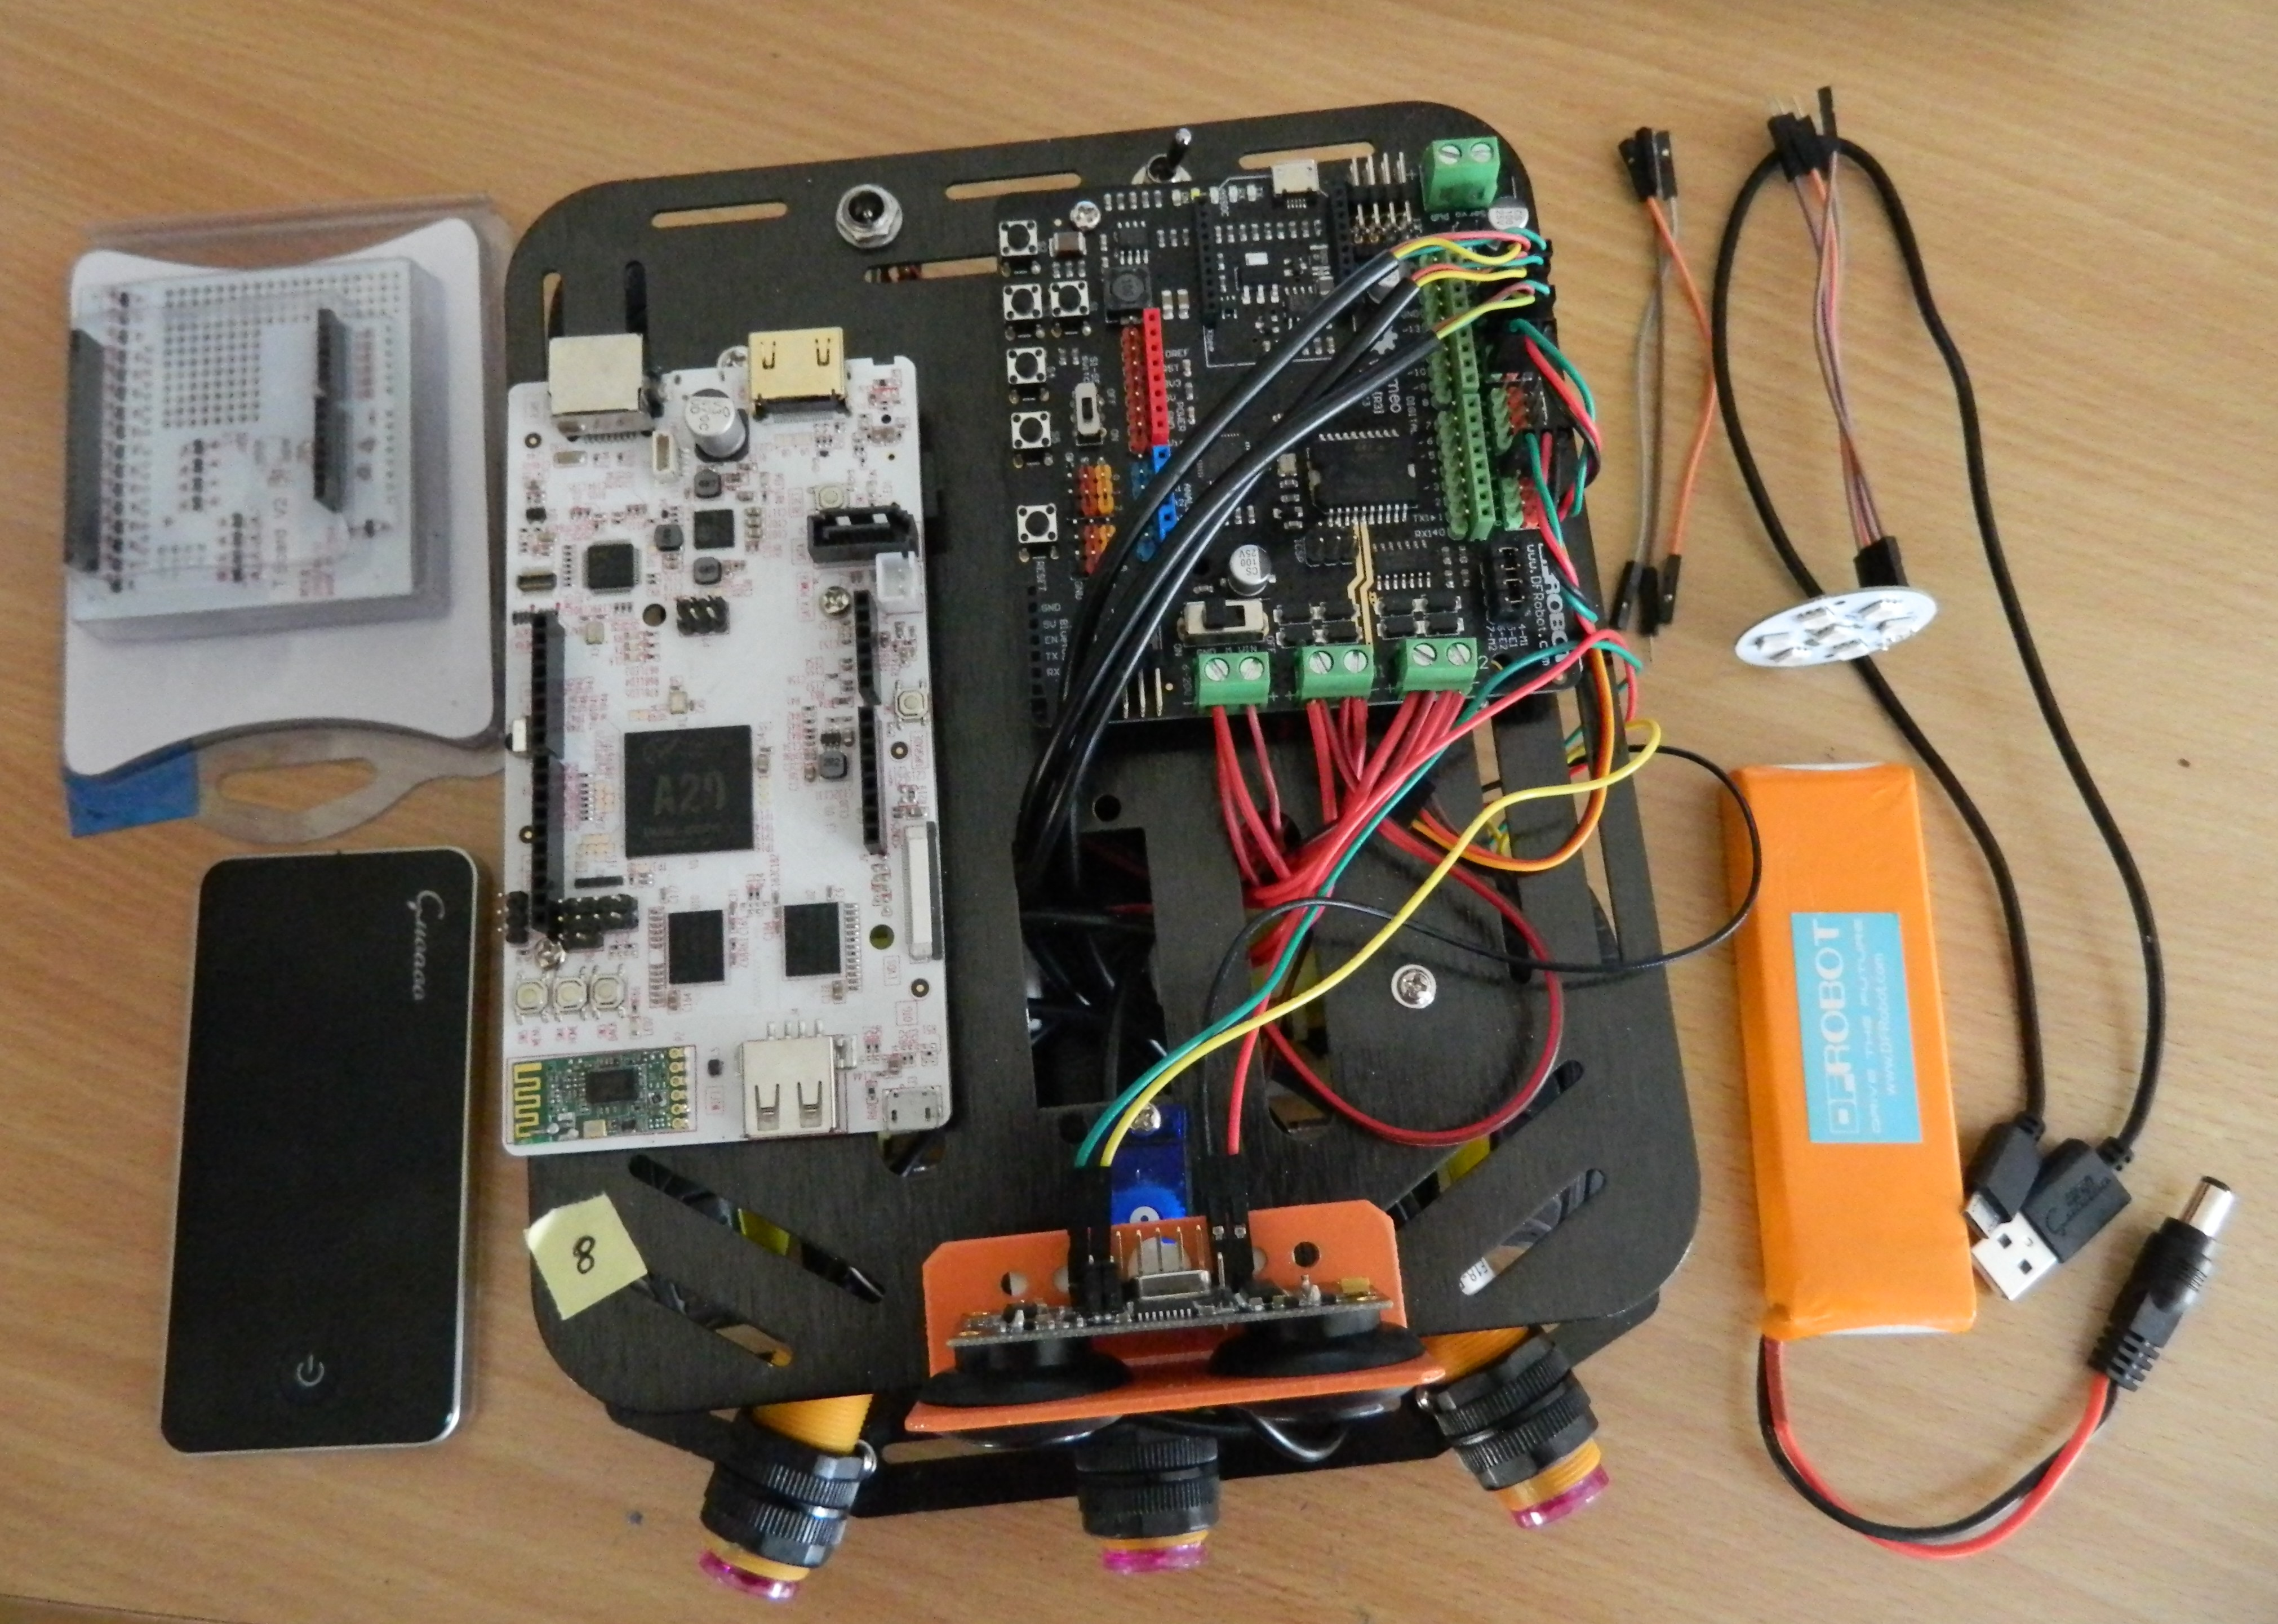
\includegraphics[scale=0.4]{./images/notre_materiel.jpg}~\
\caption{Notre materiel}
\end{figure}
	
Voici la liste du matériel dont nous disposons et dont nous devrons nous servir pour ce projet :

\begin{description}
\item [Le pcDuino :] La carte pcDuino V3 est un mini PC possédant un processeur dual core A20. Une fois branchée à un écran, un clavier et une souris, grâce à son port USB, elle s'utilise de la même manière qu'un PC sous une distribution Ubuntu. Elle possède un lecteur de carte micro-sd, car c'est dans cette carte que se situe le système d'exploitation du pcDuino. Le pcDuino posssède également un port ethernet ainsi qu'une carte wifi, ce qui permet de se connecter à un réseau facilement. Pour le faire fonctionner, il suffit de le brancher à un chargeur USB par son port micro USB. Il possède enfin des broches arduino, en plus de ses interfaces de communication, permettant de faire de la programmation arduino.\cite{ref3}
\item [L'arduino :] L'arduino Romeo V2.2 (R3) \cite{ref4} est un micro-contrôleur tout en un spécialement crée pour la robotique, qui fournit des interfaces de puissance pour contrôler des moteurs.
\item [La plateforme mobile :] Notre robot est composé d'une châssis Baron - 4WD auquel sont associées 4 moteurs reliés à 4 roues codeuses. \cite{ref5}
\item [La LED :] Le disque contient 7 LEDs RGB \cite{ref6}, que l'ont peut allumer grâce à 3 pins, un pour chaque couleur, ainsi qu'avec un pin d'alimentation.
\item [Les capteurs infrarouges :] Les 3 capteurs possèdent une LED qui s'allume si un objet est dans le champs de détection. Ils ont une sortie binaire, selon si un obstacle est détecté ou non. Leur distance de détection peut être de 3 à 80 cm, et se règle manuellement avant l'utilisation. \cite{ref7}
\item [Le capteur ultrasons :] Lié à l'arduino, il détecte des températures allant de -10 à environ 70 degrés celsius, à une distance de 4cm, jusqu'à 5m. \cite{ref8}
\end{description}

\bigskip
\begin{description}
\item [Blockly :] Nous utilisons la bibliothèque Blockly \cite{ref2} pour avoir un éditeur de code visuel. Blockly se présente sous forme de pièces de puzzle, chacune représentant un concept de code, comme une fonction, une condition, une boucle ou une variable. L'utilisateur n'a donc qu'à sélectionner et faire glisser les pièces pour les placer et les  imbriquer, afin de former un programme. Il n'a donc pas à s'occuper de la syntaxe, puisque les formes des pièces lui indique où il peut les placer ou non. Une fois le programme formé, Blockly peut le transformer en différents langages (JavaScript, Python, PHP, Dart) dont celui qui nous intéresse pour ce projet, le Lua.\\
Grâce à cette bibliothèque, nous avons la possibilité de créer les blocs de notre choix, correspondant à des fonctions à appliquer sur le robot, d'intégrer l'éditeur Blockly à notre application Androïd, et de générer le code à exécuter.
\end{description}

\chapter*{Planning}

Planning effectif jusqu'au rendu du présent rapport :\\
\begin{figure}[!h]
\begin{addmargin}[-7em]{1em}
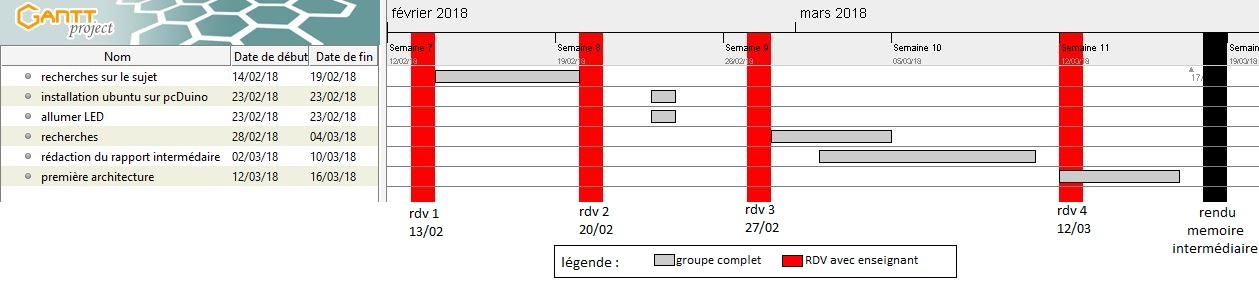
\includegraphics[scale=0.6]{./images/intermediaireEffectif.jpg}~\\[1.5cm]
\caption{Planning du 13 février au 18 mars}
\end{addmargin}
\end{figure}

Planning prévisionnel pour la suite du projet :\\


\bibliographystyle{unsrt}
\bibliography{biblio}

\end{document}
